\begin{figure}[ht] 
 	\centering 
 	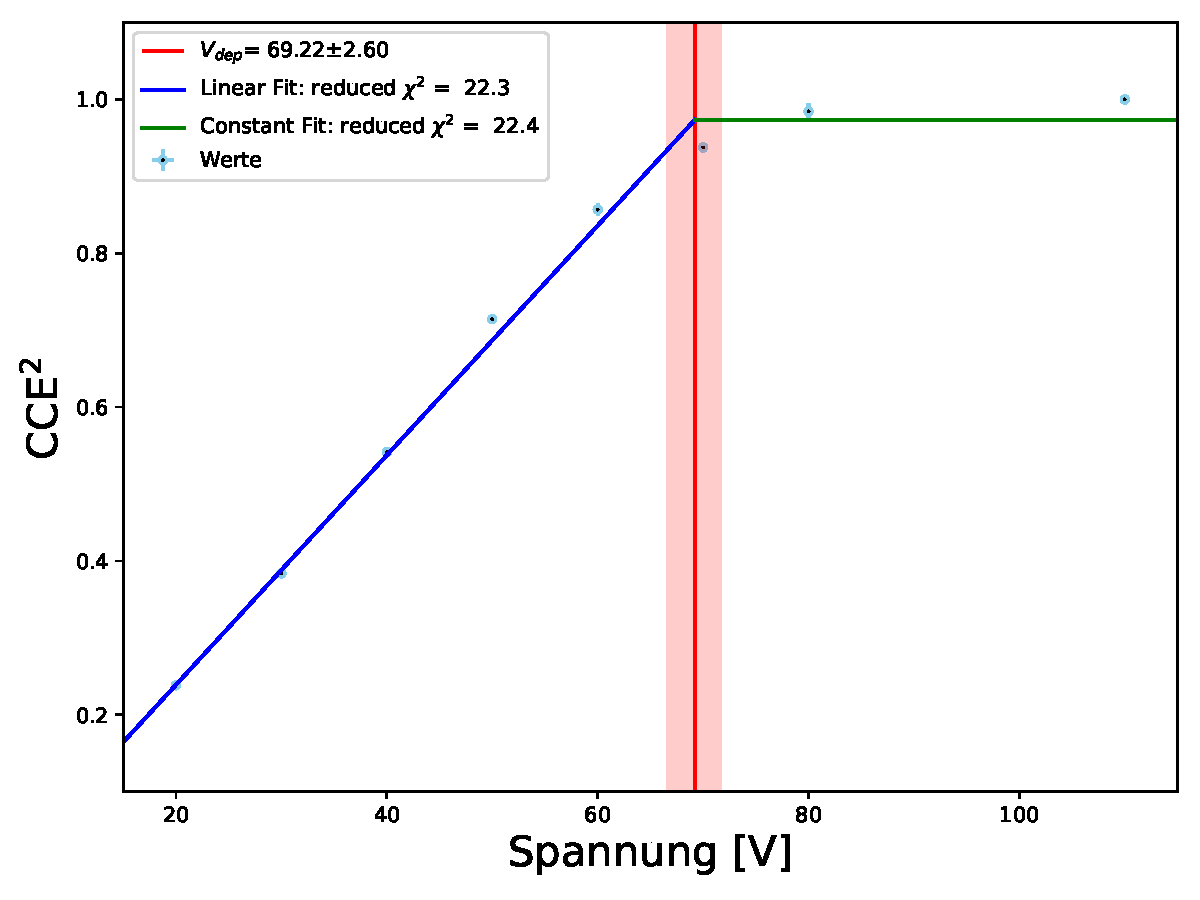
\includegraphics[width= 0.65 \textwidth]{Fits/CCE2_5_6_Fit.pdf} 
	\caption{CCE2_5_6, Fit} 
 	\label{fig:CCE2_5_6, Fit} 
\end{figure}
 \\ 
\begin{table}[ht] 
\centering 
\caption{A3_MIP_Energy.h5_charge.txt, Fit Parameter Tabelle} 
\label{tab:my-table}
\begin{tabular}{|l|c|}
\hline
Parameter Name	&	Wert \\ \hline
c	&	 0.974 \pm  0.0203\\ \hline
\end{tabular} 
\end{table}
\begin{table}[ht] 
\centering 
\caption{A3_MIP_Energy.h5_charge.txt, Fit Parameter Tabelle} 
\label{tab:my-table}
\begin{tabular}{|l|c|}
\hline
Parameter Name	&	Wert \\ \hline
slope	&	 0.0149 \pm  0.000438\\ \hline
intercept	&	-0.059688 \pm  0.0134\\ \hline
\end{tabular} 
\end{table}